\documentclass{math201}
\usepackage{hyperref}
\usepackage{bookmark}

% =============================================
% Part 0 信息
% =============================================

\mathsetup{
  % 学生姓名
  student = {},
  % 学号
  student-id = {},
  % 院系
  experiment = {PWM波形的产生},
  % 专业年级
  discipline = {集成电路设计与集成系统},
  % 日期
  date = {\today},
}

\begin{document}

% =============================================
% Part 1  封面
% =============================================

\makecover

% =============================================
% Part 2 主文档
% =============================================

\section{实验目的}

\begin{enumerate}
  \item 学习事件管理器相关基础知识,了解用通用定时器和比较单元两种方式产生PWM波。
  \item 掌握不同计数模式和输出极性下,PWM波的占空比计算方式,以及相关寄存器的参数设置。
  \item 学会认识PCB板图,找到相关的PWM波引脚。
\end{enumerate}

\section{实验要求}

本实验使用EVA的通用定时器和全比较单元产生8路PWM波形。

\subsection{输出占空比固定的PWM波形}

EVA的T1PPWM、T2PWM、PWM1/3/5输出频率为1KHz、占空比为40\%的不对称PWM波形。
PWM2/4/6输出频率为1KHz、占空比为60\%的不对称PWM波形。
各全比较单元输出的PWM波形需要具有死区,死区时间为4.27us。

\subsection{输出占空比可变的PWM波形}

PWM1和PWM2输出频率为1KHz的PWM波形。
波形的占空比每隔1s变化5\%,范围在10\%到90\%之间。死区时间为4.27us。

\section{实验原理}

\subsection{输出占空比固定的 PWM 波形}

假设需要使 EVA 的 T1PWM、T2PWM、PWM1、PWM3、PWM5 引脚输出 1kHz 、 占空比 为 40\% 的不对称 PWM 波形 PWM2 、 PWM4 、 PWM6 输出 1kHz 、 占 空 比 为 60\% 的不对称占空比为 PWM 波形; EVB 的 T3PWM、T4PWM 、 PWM7 、 PWM9 、 PWM11 引脚输出 1kHz 、 40\% 的对称 PWM 波形, PWM8 、 PWM10 、 PWM12 输出 1kHz 、 占空比为 60\% 的对称 PWM 波 形;而且各比较单元输出的 PWM 波形需要具有死区,死区时间为 4.27 μs , 那如何来实现呢?

\subsubsection{初始化系统时钟}

不管是什么样的程序,首先第 1 步需要做的就是初始化系统时钟,给整个系统分配好时钟脉冲,就像给人安上一个强有力的心脏一样。 通常 X2812 的晶振使用 30 MHz , 通过 PLL 锁相环倍频至 150MHz 。 因为需要使用到外设 EVA 和 EVB , 所以需要使能 EVA 和 EVB 的时钟。

\inputminted[
    frame=lines,
    framesep=2mm,
    baselinestretch=1.2,
    fontsize=\small,
    linenos
]{C++}{code/PWM1/DSP281x_SysCtrl.c}

\subsubsection{初始化 GPIO}

因为 F2812 的 T1PWM、T2PWM、PWM1~6、T3PWM、T4PWM、PWM7~12 引脚都是 复用的,所以需要在 GPIO 中初始化这些引脚, 使它们的功能是输出 PWM 而不是普通的数字 I/O 口。

\subsubsection{初始化事件管理器}

接下来就是初始化事件管理器模块了。 从前面 PWM 的参数和定时器寄存器之间的关系可以知道, PWM 的频率与定时器周期寄存器的值有关, PWM 的占空比与定时器比较寄存器的值有关, 当然, 这两个参数还和定时器的计数方式有关。 
下面根据例程的要求先来确定定时器周期寄存器和比较寄存器的值。

\inputminted[
    frame=lines,
    framesep=2mm,
    baselinestretch=1.2,
    fontsize=\small,
    linenos
]{C++}{code/PWM1/DSP281x_Ev.c}

\subsubsection{主函数}

最后一步, 就是任何一个工程都不能少的主函数。此处,主函数的作用主要是初始化各个模块使 DSP 稳定运行,并且启动定时器计数。

\inputminted[
    frame=lines,
    framesep=2mm,
    baselinestretch=1.2,
    fontsize=\small,
    linenos
]{C++}{code/PWM1/main.c}

\subsection{输出占空比可变的 PWM 波形}

假设 EVA 的 PWM1 和 PWM2 引脚输出频率为 1kHz 的互补的 PWM 波形, 波形 PWM 占空比每隔 1s 变化 5\% , 变化范围为 10\%~90\% , 从 10\% 不断增加至 90\% , 然后从 90\% 再不断减小至 10\% , 如此循环。 
而且 PWM1 和 PWM2 具有死区,时间为 4.27 μs 。

此处如果输出的是占空比固定的 PWM , 如是 10\% 或者 90\% , 那解决方法和前面的例程相同, 关键此处要求占空比每隔 1s 进行变化。
通过前面的学习知道, 改变 PWM 的占空比就是改变定时器比较寄存存器的值, 本例程中需要使用的是定时器 T1 和比较单元 1 , 所以也就 是需要改变 CMPR1 的值, 那如何实现每隔 1s 改变 1 次 CMPR1 的值呢?
可以利用定时器 T1 的周期中断,下面进行详细分析。

系统初始化部分和前面的一样,定时器 T1 的时钟为 37.5MHz , 此例程使得定时器 T1 工作于连续增/减计数模式。 由于 PWM 输出的频率为 1kHz 可以得到
$f = \frac{\text{TCLK} \times 10^6}{\text{T1PR} + 1} = \frac{37.5 \times 10^6}{2 \times \text{T1PR}} = 1000 Hz$
这样可以得出 T1PR = 18750, 表示成十六进制就是 0x493E。

\subsubsection{初始化系统时钟}

系统初始化模块

\inputminted[
    frame=lines,
    framesep=2mm,
    baselinestretch=1.2,
    fontsize=\small,
    linenos
]{C++}{code/PWM2/DSP281x_SysCtrl.c}

\subsubsection{初始化事件管理器}

\inputminted[
    frame=lines,
    framesep=2mm,
    baselinestretch=1.2,
    fontsize=\small,
    linenos
]{C++}{code/PWM2/DSP281x_Ev.c}

\subsubsection{主函数}

\inputminted[
    frame=lines,
    framesep=2mm,
    baselinestretch=1.2,
    fontsize=\small,
    linenos
]{C++}{code/PWM1/main.c}

\subsubsection{补充说明}

需要修改 \texttt{DSP281x\_DefaultIsr.c} 的部分代码。

\inputminted[
    frame=lines,
    framesep=2mm,
    baselinestretch=1.2,
    fontsize=\small,
    linenos
]{C++}{code/PWM2/DSP281x_DefaultIsr.c}

\section{实验步骤}

\subsection{编写代码}

\subsubsection{输出占空比固定的 PWM 波形}

修改 \texttt{common\_files/DSP2812\_sources/DSP281x\_Ev.c}

需要注意的是,教材上的代码有误,需要修改。
\texttt{EvaRegs.GPTCONA.bit.TOCMPOE = 1;} 应该修改为 \texttt{EvaRegs.GPTCONA.bit.TCMPOE = 1;}。

修改 \texttt{common\_files/DSP2812\_sources/DSP281x\_SysCtrl.c}

需要注意的是,教材上的代码有误,需要修改。
\texttt{SysCtrlRegs.PLLCR = 0xA;} 应该修改为 \texttt{SysCtrlRegs.PLLCR.all = 0xA;}。

\subsubsection{输出占空比可变的 PWM 波形}

实验发现,课本给出的代码可能不能实现PWM可变,还需要修改。

具体修改部分见 \texttt{DSP281x\_Ev.c} 和 \texttt{DSP281x\_DefaultIsr.c}。

\subsection{下载运行}

在连接示波器时,请使用杜邦线,对照原理图选择引脚。

\subsection{实验现象}

编译下载运行,实验现象如下,可以在示波器上看到波形。

查看DSP2812控制板原理图,选择PWM输出对应引脚,连接示波器,可以看到波形。

\begin{figure}[H]
  \centering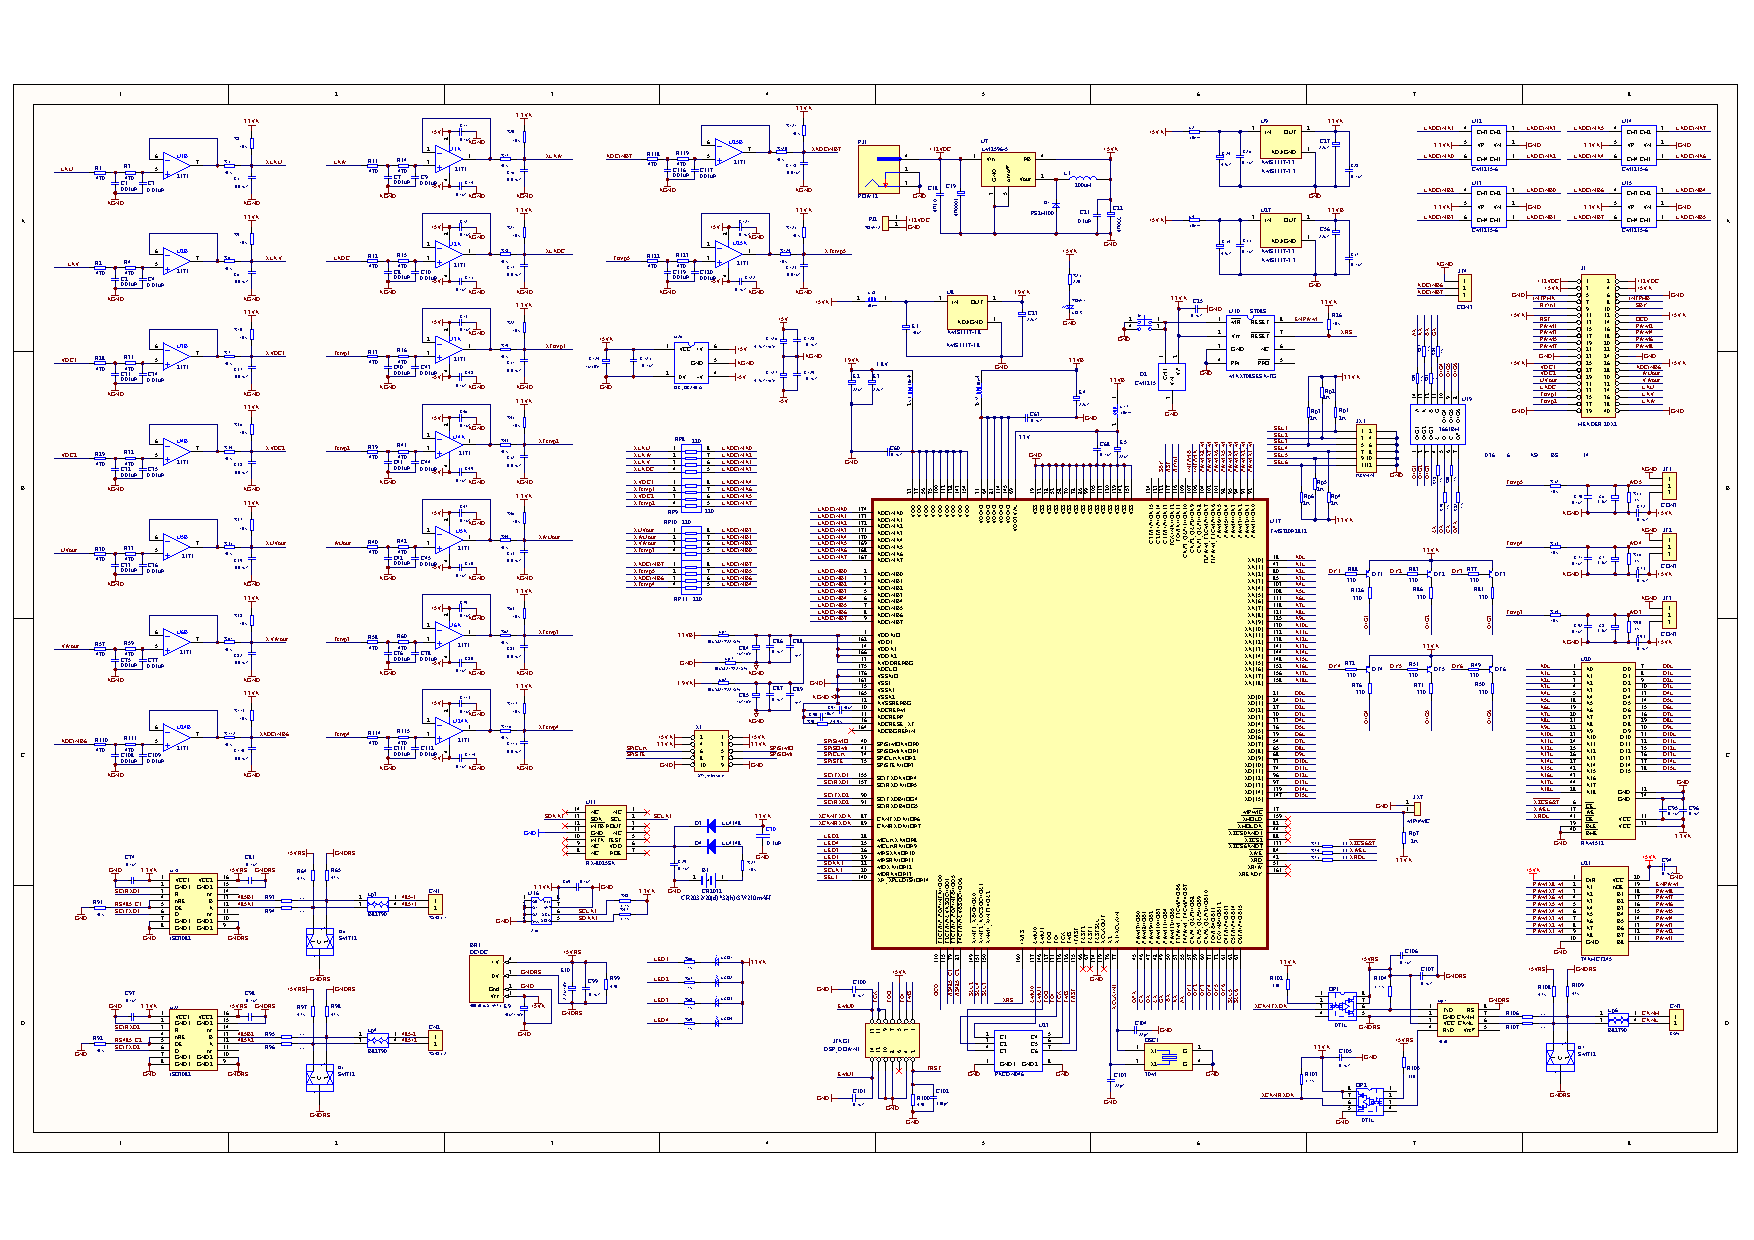
\includegraphics[page=1, trim=550 350 0 100, clip=true, width=0.8\textwidth]{DSP2812控制板原理图.pdf}
  \caption{DSP2812控制板原理图}      
\end{figure}

PWM输出对应引脚:

\begin{enumerate}
  \item PWM1: 15
  \item PWM2: 16
  \item PWM3: 17
  \item PWM4: 18
  \item PWM5: 19
  \item PWM6: 20
\end{enumerate}

\subsubsection{输出占空比固定的 PWM 波形}

\begin{figure}[H]  
  \centering\includegraphics[width=0.8\linewidth]{PWM1.jpg}  
  \caption{PWM波形1}      
\end{figure}

\begin{figure}[H]  
  \centering\includegraphics[width=0.8\linewidth]{PWM1_wire.jpg}  
  \caption{PWM波形1对应连接}      
\end{figure}

\begin{figure}[H]  
  \centering\includegraphics[width=0.8\linewidth]{PWM2.jpg}  
  \caption{PWM波形2}      
\end{figure}

\begin{figure}[H]  
  \centering\includegraphics[width=0.8\linewidth]{PWM2_wire.jpg}  
  \caption{PWM波形2对应连接}      
\end{figure}

\subsubsection{输出占空比可变的 PWM 波形}

\begin{figure}[H]  
  \centering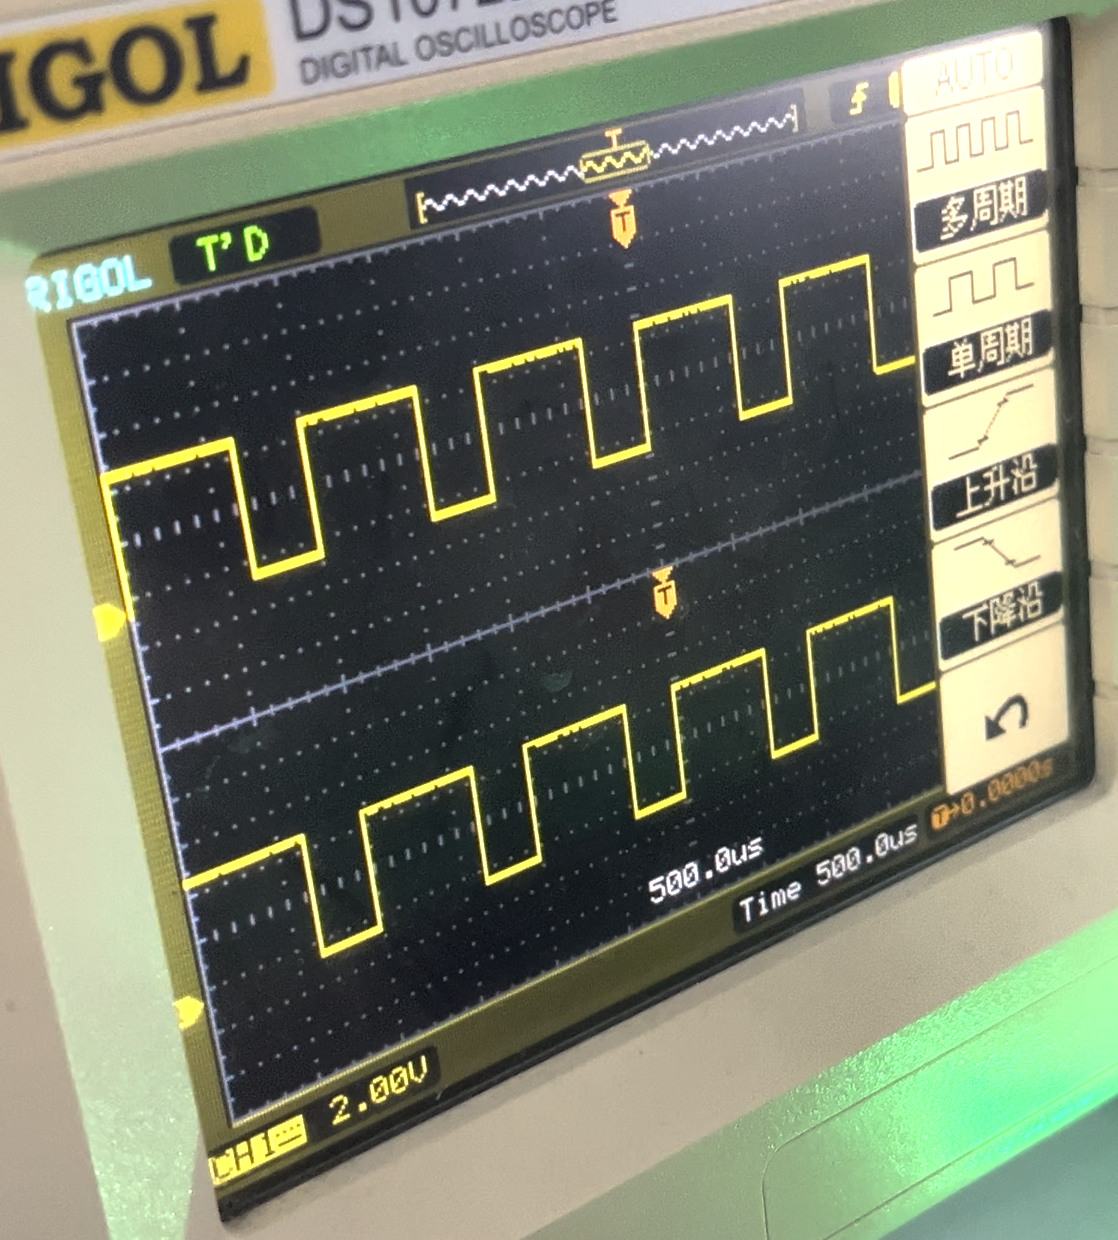
\includegraphics[width=0.8\linewidth]{PWM_change_1.png}  
  \caption{可变PWM波形1}      
\end{figure}

\section{实验小结}

通过本次实验,学习事件管理器相关基础知识,了解用通用定时器和比较单元两种方式产生PWM波;
掌握不同计数模式和输出极性下,PWM波的占空比计算方式,以及相关寄存器的参数设置;学会认识PCB板图,找到相关的PWM波引脚。
实验的要求是使用EVA的通用定时器和全比较单元产生8路PWM波形,其中包括输出占空比固定的PWM波形和输出占空比可变的PWM波形。
实验的原理没有在文本中给出。实验的步骤包括编写代码、下载运行和查看实验现象。
编写代码的过程中需要修改main.c、DSP281x\_Ev.c和DSP281x\_SysCtrl.c三个文件。
下载运行的过程中需要连接示波器,选择引脚。实验的现象是可以在示波器上看到波形。

\end{document}
